\documentclass{article}

% content/resources/templates/preamble.tex
\usepackage[margin=0.6in]{geometry}
\author{Milav Dabgar}
\usepackage{amsmath,amssymb,amsthm}
\usepackage{booktabs}
\usepackage{multirow}
\usepackage{xcolor}
\usepackage{tcolorbox}
\tcbuselibrary{breakable,skins}
\usepackage[colorlinks=true,linkcolor=blue]{hyperref}
\usepackage{titlesec}
\usepackage{enumitem}
\usepackage{tikz}
\usepackage{pgfplots}
\usepackage{circuitikz}
\usepackage[version=4]{mhchem}
\usepackage{longtable}
\usepackage{array}
\usepackage{float}
\usepackage{caption}
\usepackage{listings}

\lstset{
  basicstyle=\small\ttfamily,
  breaklines=true,
  breakatwhitespace=false,
  postbreak=\mbox{\textcolor{red}{$\hookrightarrow$}\space},
  float=false,
  numbers=left,
  numberstyle=\tiny\color{gray},
  numbersep=10pt,
  xleftmargin=2em,
  keywordstyle=\color{blue},
  commentstyle=\color{green!60!black},
  stringstyle=\color{purple},
  backgroundcolor=\color{gray!5},
  showstringspaces=false,
  tabsize=2,
  captionpos=b,
  keepspaces=true,
  columns=flexible
}

\pgfplotsset{compat=1.18}
\usetikzlibrary{shapes,arrows,positioning,calc,patterns,decorations.pathmorphing,decorations.markings,arrows.meta}

% Color scheme
\definecolor{headcolor}{RGB}{0,102,204}
\definecolor{keycolor}{RGB}{220,20,60}
\definecolor{solutioncolor}{RGB}{34,139,34}
\definecolor{mnemoniccolor}{RGB}{148,0,211}
\definecolor{codecolor}{RGB}{0,0,100}

% Spacing
\setlength{\parskip}{3pt}
\setlist[itemize]{nosep}
\setlist[enumerate]{nosep}

% Title formatting
\titleformat{\section}{\Large\bfseries\color{headcolor}}{\thesection}{1em}{}
\titleformat{\subsection}{\large\bfseries\color{headcolor}}{\thesubsection}{1em}{}

% Pandoc tightlist compatibility
\providecommand{\tightlist}{%
  \setlength{\itemsep}{0pt}\setlength{\parskip}{0pt}}

% Pandoc longtable compatibility
\newcounter{none}
\def\thenone{}


% content/resources/templates/english-boxes.tex

% Custom environments
\newtcolorbox{solutionbox}{
 breakable,
 enhanced,
 colback=solutioncolor!5!white,
 colframe=solutioncolor!75!black,
 fonttitle=\bfseries,
 title=Solution
}

\newtcolorbox{solutionboxnobreak}{
 colback=solutioncolor!5!white,
 colframe=solutioncolor!75!black,
 fonttitle=\bfseries,
 title=Solution
}

\newtcolorbox{keyformula}{
 breakable,
 enhanced,
 colback=keycolor!5!white,
 colframe=keycolor!75!black,
 fonttitle=\bfseries,
 title=Key Formula
}

\newtcolorbox{mnemonicboxenv}{
 breakable,
 enhanced,
 colback=mnemoniccolor!5!white,
 colframe=mnemoniccolor!75!black,
 fonttitle=\bfseries,
 title=Mnemonic
}

\newcommand{\mnemonicbox}[1]{%
  \begin{mnemonicboxenv}
    #1
  \end{mnemonicboxenv}
}


% Custom commands for GTU solutions
% This file defines semantic commands for consistent formatting

% Question command with automatic formatting
\newcommand{\question}[2]{%
  \section*{Question #1}%
  \textbf{#2}%
}

% OR question variant
\newcommand{\questionor}[2]{%
  \section*{Question #1 OR}%
  \textbf{#2}%
}

% Proper table environment with caption
\newenvironment{answertable}[1]{%
  \begin{table}[htbp]
  \centering
  \caption{#1}
}{%
  \end{table}
}

% Proper figure environment for diagrams
\newenvironment{answerdiagram}[1]{%
  \begin{figure}[htbp]
  \centering
  \caption{#1}
}{%
  \end{figure}
}

% Semantic markup for key terms
\newcommand{\keyword}[1]{\textbf{#1}}
\newcommand{\code}[1]{\texttt{#1}}
\newcommand{\classname}[1]{\texttt{#1}}
\newcommand{\methodname}[1]{\texttt{#1}}

% Proper quotation marks
\newcommand{\mnemonic}[1]{``#1''}


\title{Database Management (4331603) - Winter 2024 Solution}
\date{December 7, 2024}

\tikzset{
  gtu entity/.style={rectangle, draw, fill=blue!10, align=center, minimum height=2em, minimum width=3em},
  gtu relationship/.style={diamond, draw, fill=green!10, align=center, aspect=2, inner sep=1pt},
  gtu attribute/.style={ellipse, draw, fill=yellow!10, align=center, inner sep=2pt}
}

\begin{document}
\maketitle

\questionmarks{1(a)}{3}{Explain three-level database architecture.}

\begin{solutionbox}
\textbf{Table:}
\begin{center}
\captionof{table}{Database Architecture Levels}
\begin{tabulary}{\linewidth}{|L|L|L|}
\hline
\textbf{Level} & \textbf{Description} & \textbf{Purpose} \\ \hline
\textbf{External Level} & User views and application programs & Data abstraction for users \\ \hline
\textbf{Conceptual Level} & Complete logical structure & Organization-wide data view \\ \hline
\textbf{Internal Level} & Physical storage details & Storage and access methods \\ \hline
\end{tabulary}
\end{center}

\begin{center}
\begin{tikzpicture}[node distance=1.5cm, auto, thick]
    % Nodes
    \node [gtu block, fill=red!10, minimum width=6cm] (Ext) {External Level (User Views)};
    \node [gtu block, fill=blue!10, minimum width=6cm, below=1cm of Ext] (Con) {Conceptual Level (Logical Structure)};
    \node [gtu block, fill=green!10, minimum width=6cm, below=1cm of Con] (Int) {Internal Level (Physical Storage)};
    
    % Users above
    \node [above=0.8cm of Ext] (Users) {End Users / Applications};
    
    % Storage below
    \node [below=0.8cm of Int] (Storage) {Physical Database};
    
    % Connections
    \draw [gtu arrow] (Users) -- (Ext);
    \draw [gtu arrow] (Ext) -- (Con);
    \draw [gtu arrow] (Con) -- (Int);
    \draw [gtu arrow] (Int) -- (Storage);
    
    % Mappings labels
    \node [right=0.2cm of Ext, font=\small, anchor=west] {External/Conceptual Mapping};
    \node [right=0.2cm of Con, font=\small, anchor=west] {Conceptual/Internal Mapping};
\end{tikzpicture}
\captionof{figure}{Three-Level Architecture}
\end{center}

\begin{itemize}
    \item \keyword{External Level}: Individual user views and specific application requirements
    \item \keyword{Conceptual Level}: Complete database schema without storage details
    \item \keyword{Internal Level}: Physical storage structures and access paths
\end{itemize}
\end{solutionbox}

\begin{mnemonicbox}
\mnemonic{ECI - Every Computer Interface}
\end{mnemonicbox}

\questionmarks{1(b)}{4}{Explain Total Participation and Partial Participation with example.}

\begin{solutionbox}
\textbf{Table:}
\begin{center}
\captionof{table}{Participation Types}
\begin{tabulary}{\linewidth}{|L|L|L|L|}
\hline
\textbf{Participation Type} & \textbf{Definition} & \textbf{Symbol} & \textbf{Example} \\ \hline
\textbf{Total Participation} & Every entity must participate & Double line & Student-Course enrollment \\ \hline
\textbf{Partial Participation} & Some entities may not participate & Single line & Employee-Department management \\ \hline
\end{tabulary}
\end{center}

\begin{center}
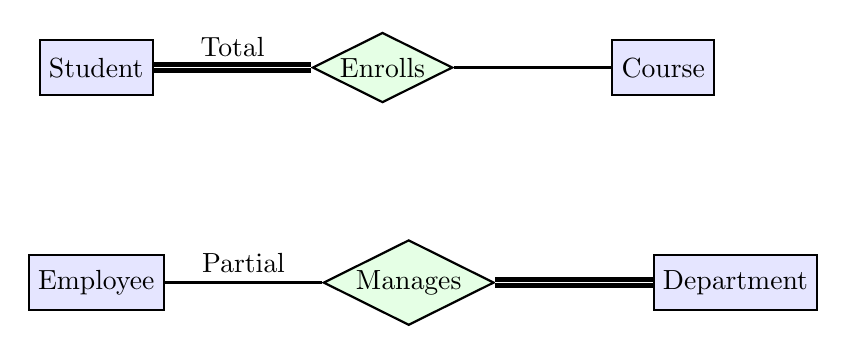
\begin{tikzpicture}[node distance=2cm, auto, thick]
    % Nodes for Total
    \node [gtu entity] (Stud) {Student};
    \node [gtu relationship, right=2cm of Stud] (Enrolls) {Enrolls};
    \node [gtu entity, right=2cm of Enrolls] (Course) {Course};
    
    % Double line for Total
    \draw [double, ultra thick] (Stud) -- (Enrolls) node[midway, above] {Total};
    \draw [thick] (Enrolls) -- (Course);
    
    % Nodes for Partial (below)
    \node [gtu entity, below=2cm of Stud] (Emp) {Employee};
    \node [gtu relationship, right=2cm of Emp] (Manages) {Manages};
    \node [gtu entity, right=2cm of Manages] (Dept) {Department};
    
    % Single line for Partial
    \draw [thick] (Emp) -- (Manages) node[midway, above] {Partial};
    \draw [double, ultra thick] (Manages) -- (Dept); % Department requires manager usually
\end{tikzpicture}
\captionof{figure}{Total vs Partial Participation}
\end{center}

\begin{itemize}
    \item \keyword{Total Participation}: All students must be enrolled in at least one course
    \item \keyword{Partial Participation}: Not all employees manage a department
    \item \keyword{Double lines} indicate total participation constraints
    \item \keyword{Single lines} show partial participation relationships
\end{itemize}
\end{solutionbox}

\begin{mnemonicbox}
\mnemonic{Total = Two lines, Partial = Plain line}
\end{mnemonicbox}

\questionmarks{1(c)}{7}{Explain advantages of DBMS over file management systems.}

\begin{solutionbox}
\textbf{Table:}
\begin{center}
\captionof{table}{Advantages of DBMS}
\begin{tabulary}{\linewidth}{|L|L|L|}
\hline
\textbf{Advantage} & \textbf{File System} & \textbf{DBMS} \\ \hline
\textbf{Data Redundancy} & High duplication & Controlled redundancy \\ \hline
\textbf{Data Inconsistency} & Common problem & Data integrity maintained \\ \hline
\textbf{Data Sharing} & Limited sharing & Concurrent access support \\ \hline
\textbf{Security} & File-level security & User-level access control \\ \hline
\textbf{Backup \& Recovery} & Manual process & Automatic mechanisms \\ \hline
\end{tabulary}
\end{center}

\begin{itemize}
    \item \keyword{Reduced Data Redundancy}: Eliminates duplicate data storage across applications
    \item \keyword{Data Consistency}: Ensures uniform data across all applications
    \item \keyword{Data Independence}: Applications independent of data structure changes
    \item \keyword{Concurrent Access}: Multiple users can access data simultaneously
    \item \keyword{Security Control}: User authentication and authorization mechanisms
    \item \keyword{Backup and Recovery}: Automatic data protection and restoration
    \item \keyword{Data Integrity}: Constraint enforcement maintains data quality
\end{itemize}
\end{solutionbox}

\begin{mnemonicbox}
\mnemonic{RDCCSBI - Really Don't Copy, Control, Secure, Backup, Integrate}
\end{mnemonicbox}

\questionmarks{1(c OR)}{7}{List out various data models. Explain any two in brief.}

\begin{solutionbox}
\textbf{Data Models List:}
\begin{itemize}
    \item Hierarchical Data Model
    \item Network Data Model  
    \item Relational Data Model
    \item Object-Oriented Data Model
    \item Entity-Relationship Model
\end{itemize}

\textbf{Table:}
\begin{center}
\captionof{table}{Relational vs Network Model}
\begin{tabulary}{\linewidth}{|L|L|L|L|}
\hline
\textbf{Model} & \textbf{Structure} & \textbf{Advantages} & \textbf{Disadvantages} \\ \hline
\textbf{Relational Model} & Tables with rows/columns & Simple, flexible & Performance overhead \\ \hline
\textbf{Network Model} & Graph with records/links & Efficient navigation & Complex structure \\ \hline
\end{tabulary}
\end{center}

\textbf{Relational Data Model}:
\begin{itemize}
    \item \keyword{Structure}: Data organized in tables (relations)
    \item \keyword{Components}: Tuples (rows), attributes (columns), domains
    \item \keyword{Operations}: Select, project, join operations available
\end{itemize}

\textbf{Network Data Model}:
\begin{itemize}
    \item \keyword{Structure}: Graph-based with owner-member relationships
    \item \keyword{Navigation}: Explicit links between record types
    \item \keyword{Flexibility}: Many-to-many relationships supported naturally
\end{itemize}
\end{solutionbox}

\begin{mnemonicbox}
\mnemonic{HNROE - Have Network Relational Object Entity}
\end{mnemonicbox}

\questionmarks{2(a)}{3}{Explain Mapping Cardinalities.}

\begin{solutionbox}
\textbf{Table:}
\begin{center}
\captionof{table}{Cardinality Types}
\begin{tabulary}{\linewidth}{|L|L|L|L|}
\hline
\textbf{Cardinality} & \textbf{Symbol} & \textbf{Description} & \textbf{Example} \\ \hline
\textbf{One-to-One} & 1:1 & Each entity relates to one other & Person-Passport \\ \hline
\textbf{One-to-Many} & 1:M & One entity relates to many & Department-Employee \\ \hline
\textbf{Many-to-One} & M:1 & Many entities relate to one & Student-Course \\ \hline
\textbf{Many-to-Many} & M:N & Many relate to many & Student-Subject \\ \hline
\end{tabulary}
\end{center}

\begin{center}
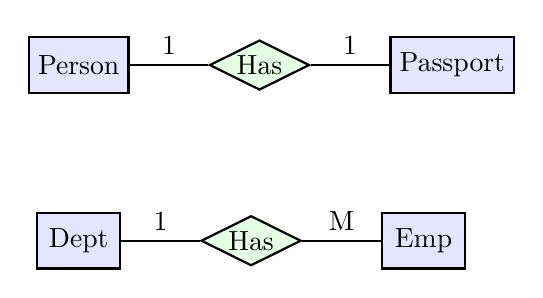
\begin{tikzpicture}[node distance=2.5cm, auto, thick]
    % 1:1
    \node [gtu entity] (P) {Person};
    \node [gtu relationship, right=1cm of P] (Has) {Has};
    \node [gtu entity, right=1cm of Has] (Pass) {Passport};
    \draw [thick] (P) -- (Has) node[midway, above] {1};
    \draw [thick] (Has) -- (Pass) node[midway, above] {1};
    
    % 1:M (Below)
    \node [gtu entity, below=1.5cm of P] (Dept) {Dept};
    \node [gtu relationship, right=1cm of Dept] (EmpIn) {Has};
    \node [gtu entity, right=1cm of EmpIn] (Emp) {Emp};
    \draw [thick] (Dept) -- (EmpIn) node[midway, above] {1};
    \draw [thick] (EmpIn) -- (Emp) node[midway, above] {M};
    
\end{tikzpicture}
\captionof{figure}{Cardinality Examples}
\end{center}

\begin{itemize}
    \item \keyword{Cardinality constraints}: define relationship participation limits
    \item \keyword{Maximum cardinality}: specifies upper bound of associations
    \item \keyword{Importance}: Helps in database design and relationship modeling
\end{itemize}
\end{solutionbox}

\begin{mnemonicbox}
\mnemonic{OMOM - One, One-Many, One-Many, Many-Many}
\end{mnemonicbox}

\questionmarks{2(b)}{4}{Explain Outer Join operation in Relational Algebra.}

\begin{solutionbox}
\textbf{Table:}
\begin{center}
\captionof{table}{Outer Join Types}
\begin{tabulary}{\linewidth}{|L|C|L|L|}
\hline
\textbf{Join Type} & \textbf{Symbol} & \textbf{Result} & \textbf{NULL Handling} \\ \hline
\textbf{Left Outer Join} & $\bowtie_L$ & All left + matching right & NULLs for unmatched right \\ \hline
\textbf{Right Outer Join} & $\bowtie_R$ & All right + matching left & NULLs for unmatched left \\ \hline
\textbf{Full Outer Join} & $\bowtie_F$ & All from both tables & NULLs for unmatched \\ \hline
\end{tabulary}
\end{center}

\textbf{Example:}
\begin{itemize}
    \item \code{EMPLOYEE LEFT OUTER JOIN DEPARTMENT}
    \item Includes all employees
    \item NULL values for employees without departments
\end{itemize}

\begin{itemize}
    \item \keyword{Preserves tuples}: Keeps unmatched tuples from specified relation(s)
    \item \keyword{NULL values}: Fills missing attribute values
    \item \keyword{Usage}: Useful for reporting incomplete data relationships
\end{itemize}
\end{solutionbox}

\begin{mnemonicbox}
\mnemonic{LRF - Left Right Full outer joins}
\end{mnemonicbox}

\questionmarks{2(c)}{7}{Explain concept of Specialization and Generalization with example.}

\begin{solutionbox}
\textbf{Table:}
\begin{center}
\captionof{table}{Specialization vs Generalization}
\begin{tabulary}{\linewidth}{|L|L|L|L|}
\hline
\textbf{Concept} & \textbf{Direction} & \textbf{Process} & \textbf{Example} \\ \hline
\textbf{Specialization} & Top-Down & General to Specific & Vehicle $\to$ Car, Truck \\ \hline
\textbf{Generalization} & Bottom-Up & Specific to General & Car, Truck $\to$ Vehicle \\ \hline
\end{tabulary}
\end{center}

\begin{center}
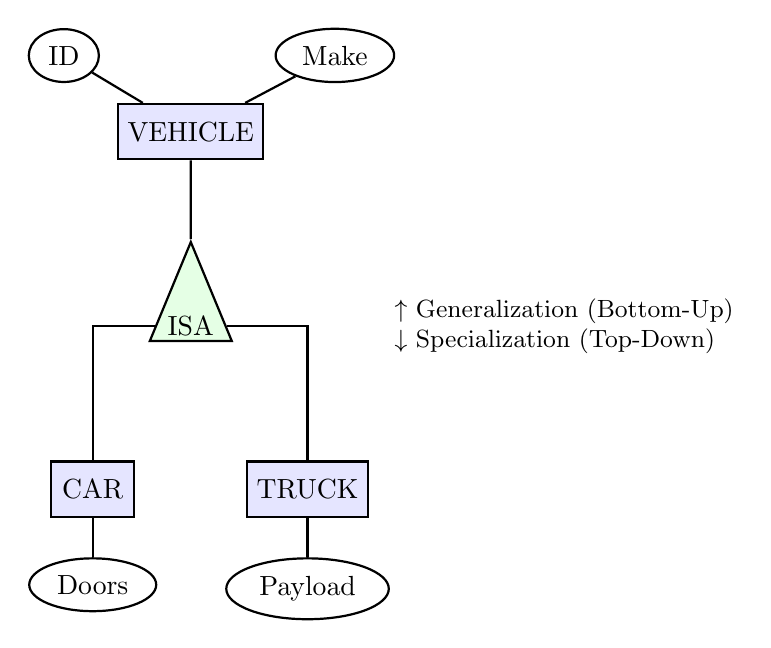
\begin{tikzpicture}[node distance=1.5cm, auto, thick]
    % Superclass
    \node [gtu entity] (Veh) {VEHICLE};
    
    % ISA Hierarchy
    \node [gtu relationship, below=1cm of Veh, isosceles triangle, shape border rotate=90, inner sep=2pt, aspect=1] (ISA) {ISA};
    
    % Subclasses
    \node [gtu entity, below left=1.5cm and 0.5cm of ISA] (Car) {CAR};
    \node [gtu entity, below right=1.5cm and 0.5cm of ISA] (Truck) {TRUCK};
    
    % Connections
    \draw [thick] (Veh) -- (ISA);
    \draw [thick] (ISA) -| (Car);
    \draw [thick] (ISA) -| (Truck);
    
    % Attributes (Optional visualization)
    % Attributes (Optional visualization)
    \node [ellipse, draw, above left=0.5cm of Veh] (ID) {ID};
    \node [ellipse, draw, above right=0.5cm of Veh] (Make) {Make};
    
    \node [ellipse, draw, below=0.5cm of Car] (Doors) {Doors};
    \node [ellipse, draw, below=0.5cm of Truck] (Payload) {Payload};
    
    \draw [thick] (Veh) -- (ID);
    \draw [thick] (Veh) -- (Make);
    \draw [thick] (Car) -- (Doors);
    \draw [thick] (Truck) -- (Payload);
    
    % Labels
    \node [right=2cm of ISA, align=left, font=\small] {$\uparrow$ Generalization (Bottom-Up)\\$\downarrow$ Specialization (Top-Down)};
\end{tikzpicture}
\captionof{figure}{ISA Hierarchy Example}
\end{center}

\textbf{Specialization:}
\begin{itemize}
    \item \keyword{Process}: Creating subclasses from superclass (Top-Down)
    \item \keyword{Inheritance}: Subclasses inherit all superclass attributes
    \item \keyword{Extension}: Subclasses have specific additional attributes
\end{itemize}

\textbf{Generalization:}
\begin{itemize}
    \item \keyword{Process}: Creating superclass from common subclass features (Bottom-Up)
    \item \keyword{Abstraction}: Identifies common attributes and relationships
    \item \keyword{Simplification}: Reduces complexity through hierarchy
\end{itemize}
\end{solutionbox}

\begin{mnemonicbox}
\mnemonic{SG-TD-BU - Specialization General-To-Detail, Bottom-Up}
\end{mnemonicbox}

\questionmarks{2(a OR)}{3}{Explain different types of Keys in Relational Algebra.}

\begin{solutionbox}
\textbf{Table:}
\begin{center}
\captionof{table}{Types of Keys}
\begin{tabulary}{\linewidth}{|L|L|L|L|}
\hline
\textbf{Key Type} & \textbf{Definition} & \textbf{Uniqueness} & \textbf{Example} \\ \hline
\textbf{Super Key} & Any attribute set that uniquely identifies & Yes & \{ID, Name, Phone\} \\ \hline
\textbf{Candidate Key} & Minimal super key & Yes & \{ID\}, \{Email\} \\ \hline
\textbf{Primary Key} & Chosen candidate key & Yes & \{StudentID\} \\ \hline
\textbf{Foreign Key} & References primary key & No & \{DeptID\} \\ \hline
\end{tabulary}
\end{center}

\begin{itemize}
    \item \keyword{Super Key}: Uniquely identifies tuples, may have extra attributes
    \item \keyword{Candidate Key}: Minimal super key without redundant attributes
    \item \keyword{Primary Key}: Selected candidate key for entity identification
    \item \keyword{Foreign Key}: Establishes referential integrity between tables
\end{itemize}
\end{solutionbox}

\begin{mnemonicbox}
\mnemonic{SCPF - Super Candidate Primary Foreign}
\end{mnemonicbox}

\questionmarks{2(b OR)}{4}{Explain types of attributes in ER-diagram with suitable example.}

\begin{solutionbox}
\textbf{Table:}
\begin{center}
\captionof{table}{Attribute Types}
\begin{tabulary}{\linewidth}{|L|L|L|L|}
\hline
\textbf{Attribute Type} & \textbf{Symbol} & \textbf{Description} & \textbf{Example} \\ \hline
\textbf{Simple} & Oval & Cannot be subdivided & Age, Name \\ \hline
\textbf{Composite} & Tree-like & Can be subdivided & Address (Street, City) \\ \hline
\textbf{Derived} & Dashed oval & Calculated from others & Age from Birth\_Date \\ \hline
\textbf{Multi-valued} & Double oval & Multiple values & Phone\_Numbers \\ \hline
\end{tabulary}
\end{center}

\begin{center}
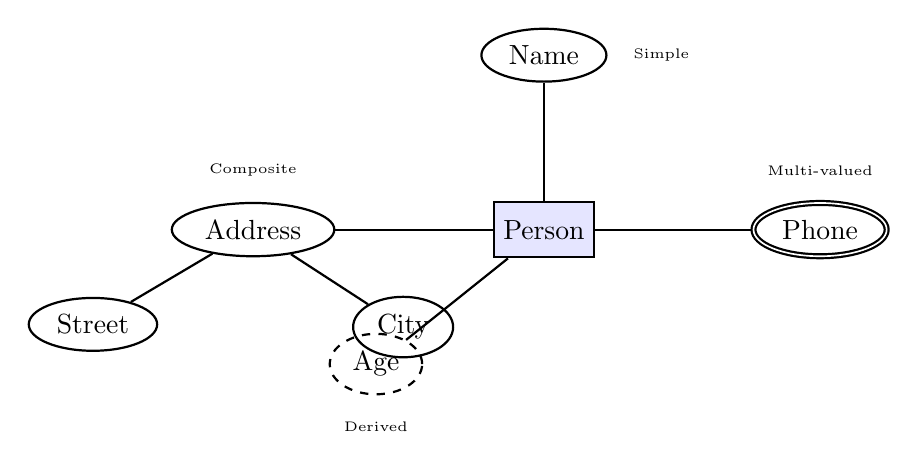
\begin{tikzpicture}[node distance=2cm, auto, thick]
    % Entity
    \node [gtu entity] (Person) {Person};
    
    % Attributes
    \node [ellipse, draw, above=1.5cm of Person] (Name) {Name};
    \node [ellipse, draw, left=2cm of Person] (Addr) {Address};
    \node [ellipse, draw, right=2cm of Person, double] (Phone) {Phone};
    \node [ellipse, draw, below left=1.5cm of Person, dashed] (Age) {Age};
    
    % Composite parts
    \node [ellipse, draw, below left=1cm of Addr] (Street) {Street};
    \node [ellipse, draw, below right=1cm of Addr] (City) {City};
    
    % Connections
    \draw [thick] (Person) -- (Name);
    \draw [thick] (Person) -- (Addr);
    \draw [thick] (Person) -- (Phone);
    \draw [thick] (Person) -- (Age);
    \draw [thick] (Addr) -- (Street);
    \draw [thick] (Addr) -- (City);
    
    % Labels
    \node [right=0.2cm of Name, font=\tiny] {Simple};
    \node [above=0.2cm of Addr, font=\tiny] {Composite};
    \node [above=0.2cm of Phone, font=\tiny] {Multi-valued};
    \node [below=0.2cm of Age, font=\tiny] {Derived};
\end{tikzpicture}
\captionof{figure}{Attribute Types in ER}
\end{center}

\begin{itemize}
    \item \keyword{Simple attributes}: atomic and indivisible
    \item \keyword{Composite attributes}: have meaningful sub-parts (e.g., Address broken into Street, City)
    \item \keyword{Derived attributes}: computed from other attribute values (e.g., Age from DOB)
    \item \keyword{Multi-valued attributes}: store multiple values per entity (e.g., Phone numbers)
\end{itemize}
\end{solutionbox}

\begin{mnemonicbox}
\mnemonic{SCDM - Simple Composite Derived Multi-valued}
\end{mnemonicbox}

\questionmarks{2(c OR)}{7}{Explain SELECT, PROJECT, UNION and SET-INTERSECTION operation with suitable example.}

\begin{solutionbox}
\textbf{Table:}
\begin{center}
\captionof{table}{Relational Operations}
\begin{tabulary}{\linewidth}{|L|C|L|L|}
\hline
\textbf{Operation} & \textbf{Symbol} & \textbf{Purpose} & \textbf{Example} \\ \hline
\textbf{SELECT} & $\sigma$ & Filter rows & $\sigma_{salary > 50000}(Employee)$ \\ \hline
\textbf{PROJECT} & $\pi$ & Select columns & $\pi_{name, age}(Employee)$ \\ \hline
\textbf{UNION} & $\cup$ & Combine relations & $R \cup S$ \\ \hline
\textbf{INTERSECTION} & $\cap$ & Common tuples & $R \cap S$ \\ \hline
\end{tabulary}
\end{center}

\textbf{1. SELECT Operation ($\sigma$):}
\begin{itemize}
    \item Filters rows based on condition.
    \item Example: $\sigma_{age > 25}(STUDENT)$
    \item Returns students older than 25 years.
\end{itemize}

\textbf{2. PROJECT Operation ($\pi$):}
\begin{itemize}
    \item Selects specific columns.
    \item Example: $\pi_{name, course}(STUDENT)$
    \item Returns only name and course columns.
\end{itemize}

\textbf{3. UNION Operation ($\cup$):}
\begin{itemize}
    \item Combines tuples from two relations (removing duplicates).
    \item Example: $SCIENCE\_STUDENTS \cup ARTS\_STUDENTS$
    \item Combines students from both streams.
\end{itemize}

\textbf{4. INTERSECTION Operation ($\cap$):}
\begin{itemize}
    \item Returns tuples present in BOTH relations.
    \item Example: $MALE\_STUDENTS \cap SPORTS\_STUDENTS$
    \item Returns male students who play sports.
\end{itemize}
\end{solutionbox}

\begin{mnemonicbox}
\mnemonic{SPUI - Select Project Union Intersection}
\end{mnemonicbox}

\questionmarks{3(a)}{3}{Differentiate Primary Key and Foreign Key constraint.}

\begin{solutionbox}
\textbf{Table:}
\begin{center}
\captionof{table}{Primary Key vs Foreign Key}
\begin{tabulary}{\linewidth}{|L|L|L|}
\hline
\textbf{Aspect} & \textbf{Primary Key} & \textbf{Foreign Key} \\ \hline
\textbf{Purpose} & Unique identification & Referential integrity \\ \hline
\textbf{NULL Values} & Not allowed & Allowed \\ \hline
\textbf{Uniqueness} & Must be unique & Can be duplicate \\ \hline
\textbf{Count} & Only one per table & Multiple allowed \\ \hline
\end{tabulary}
\end{center}

\begin{itemize}
    \item \keyword{Primary Key}: Ensures entity integrity within table (Unique + Not Null).
    \item \keyword{Foreign Key}: Maintains referential integrity between tables (links to PK).
    \item \keyword{Uniqueness}: Primary keys are always unique; foreign keys can repeat.
\end{itemize}
\end{solutionbox}

\begin{mnemonicbox}
\mnemonic{PU-FN - Primary Unique, Foreign Nullable}
\end{mnemonicbox}

\questionmarks{3(b)}{4}{Explain DUAL table and SYSDATE with example.}

\begin{solutionbox}
\textbf{Table:}
\begin{center}
\captionof{table}{DUAL and SYSDATE}
\begin{tabulary}{\linewidth}{|L|L|L|L|}
\hline
\textbf{Component} & \textbf{Type} & \textbf{Purpose} & \textbf{Example} \\ \hline
\textbf{DUAL} & Virtual table & Test expressions & \code{SELECT 2+3 FROM DUAL} \\ \hline
\textbf{SYSDATE} & System function & Current date/time & \code{SELECT SYSDATE FROM DUAL} \\ \hline
\end{tabulary}
\end{center}

\textbf{DUAL Table:}
\begin{itemize}
    \item \keyword{Virtual table}: Special one-row, one-column table present in Oracle.
    \item \keyword{Testing}: Used to select system functions or calculations not linked to a physical table.
\end{itemize}

\textbf{SYSDATE Function:}
\begin{itemize}
    \item \keyword{System Time}: Returns current date and time from the database server.
    \item \keyword{Operations}: Supports date arithmetic (e.g., \code{SYSDATE + 1} for tomorrow).
\end{itemize}

\textbf{Examples:}
\begin{itemize}
    \item \code{SELECT SYSDATE FROM DUAL;} (Current Time)
    \item \code{SELECT SYSDATE + 30 FROM DUAL;} (30 days later)
\end{itemize}
\end{solutionbox}

\begin{mnemonicbox}
\mnemonic{DT-ST - DUAL Testing, SYSDATE Time}
\end{mnemonicbox}

\questionmarks{3(c)}{7}{Write SQL queries to use various numeric functions.}

\begin{solutionbox}
\textbf{Numeric Functions Overview:}
\begin{itemize}
    \item \code{TRUNC}: Truncates number to specified precision
    \item \code{ABS}: Absolute value
    \item \code{CEIL}: Smallest integer $\geq$ n
    \item \code{FLOOR}: Largest integer $\leq$ n
    \item \code{MOD}: Remainder
    \item \code{POWER}: Exponentiation
\end{itemize}

\textbf{SQL Queries:}
\begin{itemize}
    \item (a) Display integer value of 125.25
    \newline \code{SELECT TRUNC(125.25) FROM DUAL;} $\to$ 125
    
    \item (b) Display absolute value of (-15)
    \newline \code{SELECT ABS(-15) FROM DUAL;} $\to$ 15
    
    \item (c) Display ceil value of 55.65
    \newline \code{SELECT CEIL(55.65) FROM DUAL;} $\to$ 56
    
    \item (d) Display floor value of 100.2
    \newline \code{SELECT FLOOR(100.2) FROM DUAL;} $\to$ 100
    
    \item (e) Display the square root of 16
    \newline \code{SELECT SQRT(16) FROM DUAL;} $\to$ 4
    
    \item (f) Show value of $e^3$
    \newline \code{SELECT EXP(3) FROM DUAL;}
    
    \item (g) Display result of 12 raised to 6
    \newline \code{SELECT POWER(12, 6) FROM DUAL;}
    
    \item (h) Display result of 24 mod 2
    \newline \code{SELECT MOD(24, 2) FROM DUAL;} $\to$ 0
    
    \item (i) Show output of sign(-25), sign(25), sign(0)
    \newline \code{SELECT SIGN(-25), SIGN(25), SIGN(0) FROM DUAL;} $\to$ -1, 1, 0
\end{itemize}
\end{solutionbox}

\begin{mnemonicbox}
\mnemonic{TACFSEPM - TRUNC ABS CEIL FLOOR SQRT EXP POWER MOD}
\end{mnemonicbox}

\questionmarks{3(a OR)}{3}{Explain Unique and Check Constraint with suitable example.}

\begin{solutionbox}
\textbf{Table:}
\begin{center}
\captionof{table}{Relationship Constraints}
\begin{tabulary}{\linewidth}{|L|L|L|L|}
\hline
\textbf{Constraint} & \textbf{Purpose} & \textbf{Duplicates} & \textbf{Example} \\ \hline
\textbf{UNIQUE} & Prevent duplicates & Not allowed & Email address \\ \hline
\textbf{CHECK} & Validate data & Value restrictions & Age $> 0$ \\ \hline
\end{tabulary}
\end{center}

\textbf{Examples:}
\begin{itemize}
    \item \keyword{UNIQUE Constraint}:
    \newline \code{email VARCHAR(50) UNIQUE} ensures no two students have the same email.
    
    \item \keyword{CHECK Constraint}:
    \newline \code{age NUMBER CHECK (age >= 18)} ensures age is valid.
\end{itemize}
\end{solutionbox}

\begin{mnemonicbox}
\mnemonic{UC-DV - Unique no Copy, Check Validates}
\end{mnemonicbox}

\questionmarks{3(b OR)}{4}{Explain structure of PL/SQL block.}

\begin{solutionbox}
\textbf{Table:}
\begin{center}
\captionof{table}{PL/SQL Block Sections}
\begin{tabulary}{\linewidth}{|L|L|L|L|}
\hline
\textbf{Section} & \textbf{Required} & \textbf{Purpose} & \textbf{Example} \\ \hline
\textbf{DECLARE} & Optional & Variable declarations & \code{v\_name VARCHAR2(20);} \\ \hline
\textbf{BEGIN} & Mandatory & Executable statements & \code{SELECT ... INTO ...} \\ \hline
\textbf{EXCEPTION} & Optional & Error handling & \code{WHEN OTHERS THEN ...} \\ \hline
\textbf{END} & Mandatory & Block termination & \code{END;} \\ \hline
\end{tabulary}
\end{center}

\begin{center}
\begin{tikzpicture}[node distance=0cm, auto, thick]
    \node [gtu block, minimum width=5cm, dashed] (Dec) {DECLARE (Variables)};
    \node [gtu block, minimum width=5cm, below=0cm of Dec] (Beg) {BEGIN (Logic)};
    \node [gtu block, minimum width=5cm, below=0cm of Beg, dashed] (Exc) {EXCEPTION (Errors)};
    \node [gtu block, minimum width=5cm, below=0cm of Exc] (End) {END;};
    
    % Brackets
    \draw [decorate, decoration={brace, amplitude=5pt}, thick] (Dec.north east) -- (End.south east) node [midway, right=0.5cm] {PL/SQL Block};
\end{tikzpicture}
\captionof{figure}{PL/SQL Block Structure}
\end{center}

\begin{itemize}
    \item \keyword{DECLARE section}: Variable and cursor declarations (Optional).
    \item \keyword{BEGIN-END}: Mandatory executable section containing SQL and logic.
    \item \keyword{EXCEPTION section}: Handles runtime errors (Optional).
\end{itemize}
\end{solutionbox}

\begin{mnemonicbox}
\mnemonic{DBE-E - Declare Begin Exception End}
\end{mnemonicbox}

\questionmarks{3(c OR)}{7}{Consider the following table and solve queries:}

\begin{solutionbox}
\textbf{I) Create the BRANCH table:}
\begin{lstlisting}[language=SQL]
CREATE TABLE BRANCH (
    branchid VARCHAR2(10) PRIMARY KEY,
    branchname VARCHAR2(50) NOT NULL,
    address VARCHAR2(100)
);
\end{lstlisting}

\textbf{II) Create the EMPLOYEE table:}
\begin{lstlisting}[language=SQL]
CREATE TABLE EMPLOYEE (
    empid VARCHAR2(10) PRIMARY KEY,
    name VARCHAR2(50) NOT NULL,
    post VARCHAR2(30),
    gender CHAR(1) CHECK (gender IN ('M', 'F')),
    birthdate DATE,
    salary NUMBER(10,2),
    branchid VARCHAR2(10),
    FOREIGN KEY (branchid) REFERENCES BRANCH(branchid)
);
\end{lstlisting}

\textbf{III) Find employees in Ahmedabad branch:}
\begin{lstlisting}[language=SQL]
SELECT e.* FROM EMPLOYEE e, BRANCH b 
WHERE e.branchid = b.branchid 
AND b.branchname = 'Ahmedabad';
\end{lstlisting}

\textbf{IV) Find employees born in 1998:}
\begin{lstlisting}[language=SQL]
SELECT * FROM EMPLOYEE 
WHERE EXTRACT(YEAR FROM birthdate) = 1998;
\end{lstlisting}

\textbf{V) Find female employees with salary > 5000:}
\begin{lstlisting}[language=SQL]
SELECT * FROM EMPLOYEE 
WHERE gender = 'F' AND salary > 5000;
\end{lstlisting}

\textbf{VI) Find address where Ajay works:}
\begin{lstlisting}[language=SQL]
SELECT b.address FROM EMPLOYEE e, BRANCH b
WHERE e.branchid = b.branchid 
AND e.name = 'Ajay';
\end{lstlisting}
\end{solutionbox}

\begin{mnemonicbox}
\mnemonic{CBEFFA - Create Branch Employee Find Female Address}
\end{mnemonicbox}

\questionmarks{4(a)}{3}{Explain Referential Integrity with suitable example.}

\begin{solutionbox}
\textbf{Table:}
\begin{center}
\captionof{table}{Referential Integrity}
\begin{tabulary}{\linewidth}{|L|L|L|}
\hline
\textbf{Aspect} & \textbf{Description} & \textbf{Example} \\ \hline
\textbf{Definition} & Foreign key must reference existing primary key & Employee.deptid $\to$ Department.deptid \\ \hline
\textbf{Purpose} & Maintain data consistency & Prevent orphan records \\ \hline
\textbf{Actions} & CASCADE, SET NULL, RESTRICT & ON DELETE CASCADE \\ \hline
\end{tabulary}
\end{center}

\begin{center}
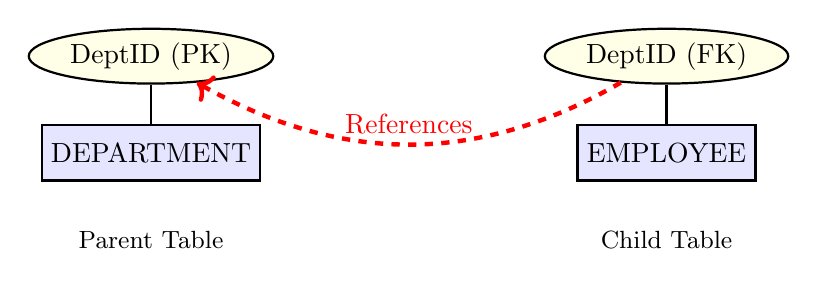
\begin{tikzpicture}[node distance=2.5cm, auto, thick]
    % Parent Rule
    \node [gtu entity] (Dept) {DEPARTMENT};
    \node [gtu attribute, above=0.5cm of Dept] (DPK) {DeptID (PK)};
    \draw [thick] (Dept) -- (DPK);
    
    % Child Rule
    \node [gtu entity, right=4cm of Dept] (Emp) {EMPLOYEE};
    \node [gtu attribute, above=0.5cm of Emp] (EFK) {DeptID (FK)};
    \draw [thick] (Emp) -- (EFK);
    
    % Reference Arrow
    \draw [->, red, dashed, ultra thick] (EFK) to[bend left] node[midway, above] {References} (DPK);
    
    % Labels
    \node [below=0.5cm of Dept, font=\small] {Parent Table};
    \node [below=0.5cm of Emp, font=\small] {Child Table};
\end{tikzpicture}
\captionof{figure}{Foreign Key Reference}
\end{center}

\begin{itemize}
    \item \keyword{Referential integrity}: ensures valid relationships between tables.
    \item \keyword{Orphan records}: prevented; cannot add employee to non-existent department.
    \item \keyword{Cascade}: operations automatically propagate updates/deletes.
\end{itemize}
\end{solutionbox}

\begin{mnemonicbox}
\mnemonic{RIO - Referential Integrity prevents Orphans}
\end{mnemonicbox}

\questionmarks{4(b)}{4}{Differentiate Partial and Full Functional Dependency.}

\begin{solutionbox}
\textbf{Table:}
\begin{center}
\captionof{table}{Dependency Types}
\begin{tabulary}{\linewidth}{|L|L|L|L|}
\hline
\textbf{Type} & \textbf{Definition} & \textbf{Example} & \textbf{Requirement} \\ \hline
\textbf{Partial} & Depends on part of composite key & (StudentID, CourseID) $\to$ Name & Composite primary key \\ \hline
\textbf{Full} & Depends on entire key & (StudentID, CourseID) $\to$ Grade & Complete key needed \\ \hline
\end{tabulary}
\end{center}

\textbf{Example:} Key is (StudentID, CourseID)
\begin{itemize}
    \item \keyword{Partial}: StudentName depends only on StudentID. Violates 2NF.
    \item \keyword{Full}: Grade depends on BOTH StudentID and CourseID. Good.
\end{itemize}

\begin{itemize}
    \item \keyword{Partial dependency} causes data redundancy and anomalies.
    \item \keyword{2NF eliminates} partial functional dependencies.
\end{itemize}
\end{solutionbox}

\begin{mnemonicbox}
\mnemonic{PF-CF - Partial Few, Complete Full}
\end{mnemonicbox}

\questionmarks{4(c)}{7}{Explain 3rd Normal Form with example.}

\begin{solutionbox}
\textbf{3rd Normal Form Requirements:}
\begin{itemize}
    \item Must be in 2NF.
    \item No transitive dependencies (Non-key $\to$ Non-key).
    \item Non-key attributes depend ONLY on the primary key.
\end{itemize}

\textbf{Problem (Before 3NF):}
\begin{center}
\begin{tabular}{|l|l|l|l|l|l|}
\hline
\textbf{StudID} & \textbf{Name} & \textbf{CourseID} & \textbf{CName} & \textbf{InstID} & \textbf{InstName} \\ \hline
S1 & John & C1 & Math & I1 & Dr. Smith \\ \hline
\end{tabular}
\end{center}
\textit{Issue: StudentID $\to$ InstID $\to$ InstName (Transitive Dependency)}

\textbf{3NF Solution (Decomposition):}

\textbf{1. STUDENT Table:}
\begin{tabular}{|l|l|l|}
\hline
\textbf{StudID} & \textbf{Name} & \textbf{CourseID} \\ \hline
S1 & John & C1 \\ \hline
\end{tabular}

\textbf{2. COURSE Table:}
\begin{tabular}{|l|l|l|}
\hline
\textbf{CourseID} & \textbf{CName} & \textbf{InstID} \\ \hline
C1 & Math & I1 \\ \hline
\end{tabular}

\textbf{3. INSTRUCTOR Table:}
\begin{tabular}{|l|l|}
\hline
\textbf{InstID} & \textbf{InstName} \\ \hline
I1 & Dr. Smith \\ \hline
\end{tabular}
\end{solutionbox}

\begin{mnemonicbox}
\mnemonic{3NF-NT - 3rd Normal Form No Transitives}
\end{mnemonicbox}

\questionmarks{4(a OR)}{3}{Explain Importance of Normalization.}

\begin{solutionbox}
\textbf{Table:}
\begin{center}
\captionof{table}{Benefits of Normalization}
\begin{tabulary}{\linewidth}{|L|L|L|}
\hline
\textbf{Benefit} & \textbf{Problem Solved} & \textbf{Result} \\ \hline
\textbf{Reduce Redundancy} & Duplicate data & Storage efficiency \\ \hline
\textbf{Eliminate Anomalies} & Update/Insert/Delete issues & Data consistency \\ \hline
\textbf{Improve Integrity} & Data inconsistency & Reliable information \\ \hline
\end{tabulary}
\end{center}

\begin{itemize}
    \item \keyword{Minimizes redundancy}: Saves storage by storing data once.
    \item \keyword{Prevents anomalies}: Ensures logical data modification.
    \item \keyword{Simplifies maintenance}: Organized structure is easier to manage.
\end{itemize}
\end{solutionbox}

\begin{mnemonicbox}
\mnemonic{RESIM - Redundancy Eliminated, Storage Improved, Maintenance}
\end{mnemonicbox}

\questionmarks{4(b OR)}{4}{Differentiate Prime Attributes and Non-Prime Attributes.}

\begin{solutionbox}
\textbf{Table:}
\begin{center}
\captionof{table}{Prime vs Non-Prime Attributes}
\begin{tabulary}{\linewidth}{|L|L|L|L|}
\hline
\textbf{Type} & \textbf{Definition} & \textbf{Role} & \textbf{Example} \\ \hline
\textbf{Prime} & Part of candidate key & Key formation & StudentID, CourseID \\ \hline
\textbf{Non-Prime} & Not part of any key & Data storage & Name, Grade \\ \hline
\end{tabulary}
\end{center}

\textbf{Example:} Relation(StudentID, CourseID, Grade, Semester)
\begin{itemize}
    \item Candidate Key: (StudentID, CourseID)
    \item \keyword{Prime Attributes}: StudentID, CourseID
    \item \keyword{Non-Prime Attributes}: Grade, Semester
\end{itemize}

\begin{itemize}
    \item \keyword{Significance}: Functional dependency involving non-prime attributes determines Normal Form (2NF/3NF).
\end{itemize}
\end{solutionbox}

\begin{mnemonicbox}
\mnemonic{PN-KD - Prime in Key, Non-prime for Data}
\end{mnemonicbox}

\questionmarks{4(c OR)}{7}{Explain 2nd Normal Form with example.}

\begin{solutionbox}
\textbf{2nd Normal Form Requirements:}
\begin{itemize}
    \item Must be in 1NF.
    \item No partial functional dependencies.
    \item Non-key attributes must depend on the WHOLE primary key.
\end{itemize}

\textbf{Problem (Before 2NF):}
\begin{center}
\begin{tabular}{|l|l|l|l|l|}
\hline
\textbf{StudID} & \textbf{CourseID} & \textbf{SName} & \textbf{CName} & \textbf{Grade} \\ \hline
S1 & C1 & John & Math & A \\ \hline
S1 & C2 & John & Physics & B \\ \hline
\end{tabular}
\end{center}
\textit{Issue: StudID $\to$ SName (Partial), CourseID $\to$ CName (Partial)}

\textbf{2NF Solution (Decomposition):}

\textbf{1. STUDENT Table:}
\begin{tabular}{|l|l|}
\hline
\textbf{StudID} & \textbf{SName} \\ \hline
S1 & John \\ \hline
\end{tabular}

\textbf{2. COURSE Table:}
\begin{tabular}{|l|l|}
\hline
\textbf{CourseID} & \textbf{CName} \\ \hline
C1 & Math \\ \hline
\end{tabular}

\textbf{3. ENROLLMENT Table:}
\begin{tabular}{|l|l|l|}
\hline
\textbf{StudID} & \textbf{CourseID} & \textbf{Grade} \\ \hline
S1 & C1 & A \\ \hline
S1 & C2 & B \\ \hline
\end{tabular}
\end{solutionbox}

\begin{mnemonicbox}
\mnemonic{2NF-FD - 2nd Normal Form Full Dependencies}
\end{mnemonicbox}

\questionmarks{5(a)}{3}{Explain Transaction states with proper diagram.}

\begin{solutionbox}
\begin{center}
\begin{tikzpicture}[node distance=2cm, auto, thick]
    % States
    \node [gtu state] (Active) {Active};
    \node [gtu state, right=2.5cm of Active] (Part) {Partially Committed};
    \node [gtu state, right=2.5cm of Part] (Comm) {Committed};
    \node [gtu state, below=1.5cm of Active] (Fail) {Failed};
    \node [gtu state, right=2.5cm of Fail] (Abort) {Aborted};
    
    % Transitions
    \draw [gtu arrow] (Active) -- (Part) node[midway, above, font=\tiny] {read/write};
    \draw [gtu arrow] (Part) -- (Comm) node[midway, above, font=\tiny] {commit};
    \draw [gtu arrow] (Active) -- (Fail) node[midway, right, font=\tiny] {error};
    \draw [gtu arrow] (Part) -- (Fail) node[midway, right, font=\tiny] {error};
    \draw [gtu arrow] (Fail) -- (Abort) node[midway, above, font=\tiny] {rollback};
\end{tikzpicture}
\captionof{figure}{Transaction State Diagram}
\end{center}

\textbf{Table:}
\begin{center}
\captionof{table}{Transaction States}
\begin{tabulary}{\linewidth}{|L|L|L|}
\hline
\textbf{State} & \textbf{Description} & \textbf{Next State} \\ \hline
\textbf{Active} & Executing operations & Partial/Failed \\ \hline
\textbf{Partially Committed} & Last statement executed & Committed/Failed \\ \hline
\textbf{Committed} & Successful completion & End \\ \hline
\textbf{Failed} & Execution stopped due to error & Aborted \\ \hline
\textbf{Aborted} & Rolling back changes & End \\ \hline
\end{tabulary}
\end{center}
\end{solutionbox}

\begin{mnemonicbox}
\mnemonic{APCFA - Active Partial Commit Fail Abort}
\end{mnemonicbox}

\questionmarks{5(b)}{4}{Explain any two DDL commands with a suitable example.}

\begin{solutionbox}
\textbf{Table:}
\begin{center}
\captionof{table}{DDL Commands}
\begin{tabulary}{\linewidth}{|L|L|L|L|}
\hline
\textbf{Command} & \textbf{Purpose} & \textbf{Example Syntax} \\ \hline
\textbf{CREATE} & Create objects & \code{CREATE TABLE T (...)} \\ \hline
\textbf{ALTER} & Modify structure & \code{ALTER TABLE T ADD ...} \\ \hline
\end{tabulary}
\end{center}

\textbf{1. CREATE Command:}
\begin{lstlisting}[language=SQL]
CREATE TABLE EMPLOYEE (
    empid NUMBER(5) PRIMARY KEY,
    name VARCHAR2(50)
);
\end{lstlisting}

\textbf{2. ALTER Command:}
\begin{lstlisting}[language=SQL]
-- Add new column
ALTER TABLE EMPLOYEE ADD phone VARCHAR2(15);
-- Modify column
ALTER TABLE EMPLOYEE MODIFY name VARCHAR2(100);
-- Drop column
ALTER TABLE EMPLOYEE DROP COLUMN phone;
\end{lstlisting}

\begin{itemize}
    \item \keyword{DDL}: Data Definition Language defines schema.
    \item \keyword{Auto-commit}: DDL commands are automatically saved.
\end{itemize}
\end{solutionbox}

\begin{mnemonicbox}
\mnemonic{CA-NM - CREATE Adds, ALTER Modifies}
\end{mnemonicbox}

\questionmarks{5(c)}{7}{Explain ACID Properties in detail.}

\begin{solutionbox}
\textbf{Table:}
\begin{center}
\captionof{table}{ACID Properties}
\begin{tabulary}{\linewidth}{|L|L|L|}
\hline
\textbf{Property} & \textbf{Definition} & \textbf{Example} \\ \hline
\textbf{Atomicity} & All or nothing & Complete transfer or rollback \\ \hline
\textbf{Consistency} & Database always valid & Balance never negative \\ \hline
\textbf{Isolation} & Independent execution & Concurrent users don't interfere \\ \hline
\textbf{Durability} & Permanent changes & Data survives power loss \\ \hline
\end{tabulary}
\end{center}

\begin{itemize}
    \item \keyword{Atomicity}: Transaction is an indivisible unit.
    \item \keyword{Consistency}: Transforms DB from one valid state to another.
    \item \keyword{Isolation}: Intermediate states are invisible to other transactions.
    \item \keyword{Durability}: Committed data is saved permanently even after crash.
\end{itemize}
\end{solutionbox}

\begin{mnemonicbox}
\mnemonic{ACID - Atomicity Consistency Isolation Durability}
\end{mnemonicbox}

\questionmarks{5(a OR)}{3}{What is two phase locking technique?}

\begin{solutionbox}
\textbf{Table:}
\begin{center}
\captionof{table}{2PL Phases}
\begin{tabulary}{\linewidth}{|L|L|L|L|}
\hline
\textbf{Phase} & \textbf{Action} & \textbf{Description} & \textbf{Allowed} \\ \hline
\textbf{Growing} & Acquire locks & Transaction obtains all locks & LOCK \\ \hline
\textbf{Shrinking} & Release locks & Transaction releases locks & UNLOCK \\ \hline
\end{tabulary}
\end{center}

\begin{center}
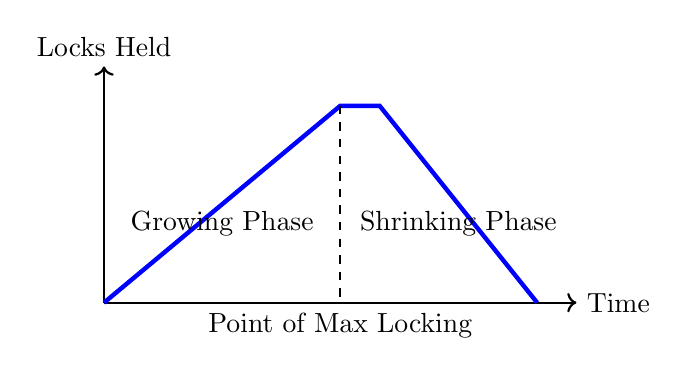
\begin{tikzpicture}[thick]
    % Axes
    \draw [->] (0,0) -- (6,0) node[right] {Time};
    \draw [->] (0,0) -- (0,3) node[above] {Locks Held};
    
    % Graph line
    \draw [blue, ultra thick] (0,0) -- (3,2.5) -- (3.5, 2.5) -- (5.5, 0);
    
    % Checkpoints
    \draw [dashed] (3,2.5) -- (3,0) node[below] {Point of Max Locking};
    
    % Labels
    \node at (1.5, 1) {Growing Phase};
    \node at (4.5, 1) {Shrinking Phase};
\end{tikzpicture}
\captionof{figure}{Two-Phase Locking Protocol}
\end{center}

\begin{itemize}
    \item \keyword{Growing Phase}: Transaction may obtain locks, but cannot release any.
    \item \keyword{Shrinking Phase}: Transaction may release locks, but cannot obtain any.
    \item \keyword{Guarantee}: Ensures serializability.
\end{itemize}
\end{solutionbox}

\begin{mnemonicbox}
\mnemonic{2PL-GS - Two Phase Locking Growing Shrinking}
\end{mnemonicbox}

\questionmarks{5(b OR)}{4}{Explain any two DML commands with a suitable example.}

\begin{solutionbox}
\textbf{Table:}
\begin{center}
\captionof{table}{DML Commands}
\begin{tabulary}{\linewidth}{|L|L|L|}
\hline
\textbf{Command} & \textbf{Purpose} & \textbf{Example} \\ \hline
\textbf{INSERT} & Add new records & \code{INSERT INTO Student...} \\ \hline
\textbf{UPDATE} & Modify records & \code{UPDATE Student SET...} \\ \hline
\end{tabulary}
\end{center}

\textbf{1. INSERT Command:}
\begin{lstlisting}[language=SQL]
INSERT INTO EMPLOYEE (empid, name, salary)
VALUES (101, 'John Smith', 50000);
\end{lstlisting}

\textbf{2. UPDATE Command:}
\begin{lstlisting}[language=SQL]
UPDATE EMPLOYEE 
SET salary = 60000 
WHERE empid = 101;
\end{lstlisting}

\begin{itemize}
    \item \keyword{DML}: Data Manipulation Language manages data values.
    \item \keyword{Explicit Commit}: Changes often need \code{COMMIT} to be saved.
\end{itemize}
\end{solutionbox}

\begin{mnemonicbox}
\mnemonic{IU-AM - INSERT Adds, UPDATE Modifies}
\end{mnemonicbox}

\questionmarks{5(c OR)}{7}{List problems of concurrency control and explain any two in detail.}

\begin{solutionbox}
\textbf{Problems List:}
\begin{enumerate}
    \item Lost Update Problem
    \item Dirty Read Problem
    \item Non-repeatable Read Problem
    \item Phantom Read Problem
\end{enumerate}

\textbf{1. Lost Update Problem:}
\begin{itemize}
    \item \keyword{Scenario}: Two transactions update the same item, and one update overwrites the other.
    \item \keyword{Example}:
        \begin{itemize}
            \item T1 reads X=100. T2 reads X=100.
            \item T1 writes X=110. T2 writes X=90.
            \item T1's update is lost. Final X=90 (should be 100).
        \end{itemize}
\end{itemize}

\textbf{2. Dirty Read Problem:}
\begin{itemize}
    \item \keyword{Scenario}: Reading data written by an uncommitted transaction.
    \item \keyword{Example}:
        \begin{itemize}
            \item T1 updates X=200. T2 reads X=200.
            \item T1 fails and rolls back X=100.
            \item T2 has processed invalid data (200).
        \end{itemize}
\end{itemize}

\textbf{Solutions:}
\begin{itemize}
    \item Use \keyword{Locking Protocols} (2PL).
    \item Use \keyword{Isolation Levels} (Read Committed, Serializable).
\end{itemize}
\end{solutionbox}

\begin{mnemonicbox}
\mnemonic{LDUI - Lost Dirty Unrepeatable Inconsistent}
\end{mnemonicbox}

\end{document}
